\section*{1. Assignment 3.1}
\textbf{Read and understand the papers from Zhang and Heikkil (provided in LEA). Based on your understanding of camera calibration, design a calibration setup and detail the actual calibration process. \\
Test the provided camera on your laptop and ensure you can capture still images.}

\begin{figure}[H]
\begin{center}
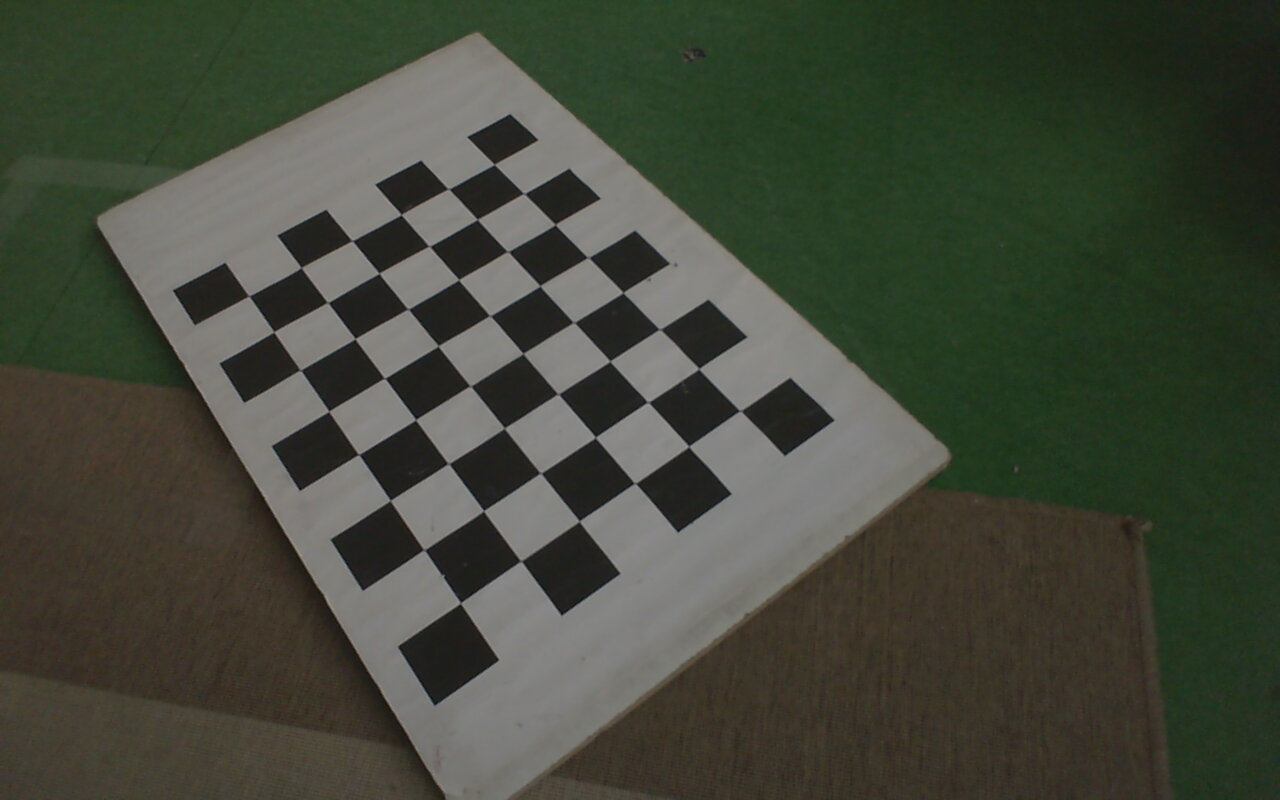
\includegraphics[width=0.7\textwidth]{data/1.jpg}
\caption{Sample image}
\label{fig:sample}
\end{center}
\end{figure}
We used VLC player to disable the auto-focussing function that is in-built in the camera. The example image is shown in fig. \ref{fig:sample}.

\section*{2. Deliverables 3.1}
\textbf{Write a design report describing the calibration process, including a theoretical part that describes the camera and lens errors measured and corrected by the calibration. Your design report should cover:}

\subsection*{1. A description of the setup for calibration, including possible pitfalls}

\subsection*{2. An estimation of the number of images and image positions required}
We used 51 images. For calibration procedure not all images are needed however we use all the images for the camera calibration.

\subsection*{3. A description of the parameters (what do they mean?) calculated by the Matlab calibration toolbox}

\subsection*{4. Discuss possible problems or error sources that can disturb the calibration process. Include any observation you may have made while testing the proper functioning of the camera with your laptop}

\section*{3. Assignment 3.2}
\subsection*{Perform the camera calibration experiment designed in assignment 3.1. Document all relevant aspects needed to assess the quality of your obtained camera parameters.}

\section*{4. Deliverables 3.2}
\textbf{Write a report describing the calibration process, including a theoretical part that describes the camera and lens errors measured and corrected by the calibration:}
\subsection*{1. Describe the images poses used for calibration and report the found camera parameters including any error estimates (where applicable)}
\begin{figure}[H]
\begin{center}
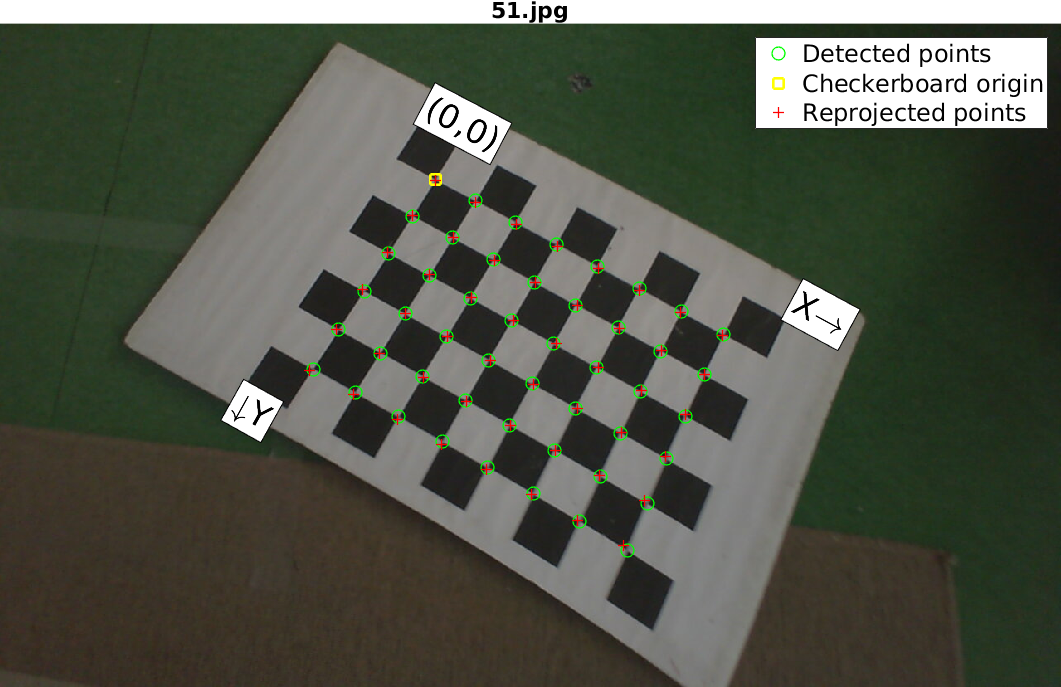
\includegraphics[width=0.7\textwidth]{graphics/worst.png}
\caption{Calibrated image with the highest amount of pixel error}
\label{fig:worst-calibrated-image}
\end{center}
\end{figure}

\begin{figure}[H]
\begin{center}
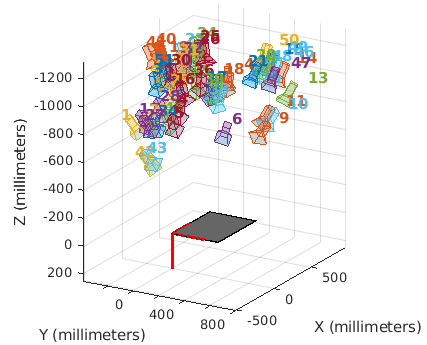
\includegraphics[width=0.7\textwidth]{graphics/camera_positions.png}
\caption{Camera positions evaluated via calibration procedure.}
\label{fig:poses}
\end{center}
\end{figure}

\begin{figure}[H]
\begin{center}
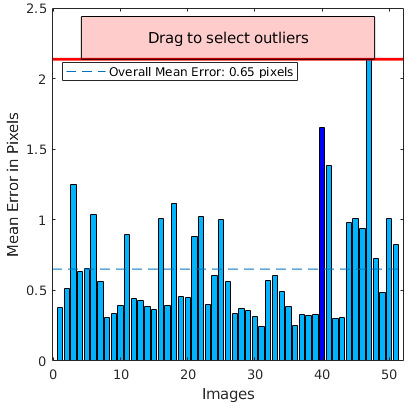
\includegraphics[width=0.7\textwidth]{graphics/stats.png}
\caption{Mean error in Pixels for each image.}
\label{fig:stats}
\end{center}
\end{figure}
\subsection*{2. Provide arguments for which camera model best fits your situation and hence should be used}

\subsection*{3. Discuss possible problems or error sources that can disturb the calibration process}
%%%%%%%%%%%%%%%%%%%%%%%%%%%%%%%%%%%%%%%%%%%%%%%%%%%%%%%%%%%%%%%%%%%%%%%%%%%%%